\subsection{Descripción del problema.}

\vspace*{0.3cm}

En este problema, un cliente busca ofrecer un servicio particular sobre una
red existente de computadoras. Nuestra tarea consiste en elegir algunas de las
mismas, para utilizarlas como servidores formando un \textit{backbone} que
siga una tipología de red de tipo \textit{anillo}. Además, se requiere que
las demás computadoras de la red estén conectadas a algún servidor
perteneciente a este anillo, para poder tener acceso al mismo.

La red cuenta con conexiones entre algunos pares de equipos, pero
\textbf{por cada conexión utilizada se deberá pagar cierto costo
asociado al enlace utilizado}.

\medskip

El objetivo es elegir el anillo de servidores (indicando qué servidores y
enlaces lo representarán) y todas las demás conexiones necesarias, de
manera tal que las demás computadoras queden conectadas al anillo y el costo
asociado al uso de estos enlaces sea \textbf{mínimo}.

\vspace*{0.5cm}

\textbf{Ejemplo:}

En un sistema con 11 computadoras unidas con 13 enlaces distribuidas como
muestra la siguiente imagen:

\begin{figure}[htb]
  \begin{center}
      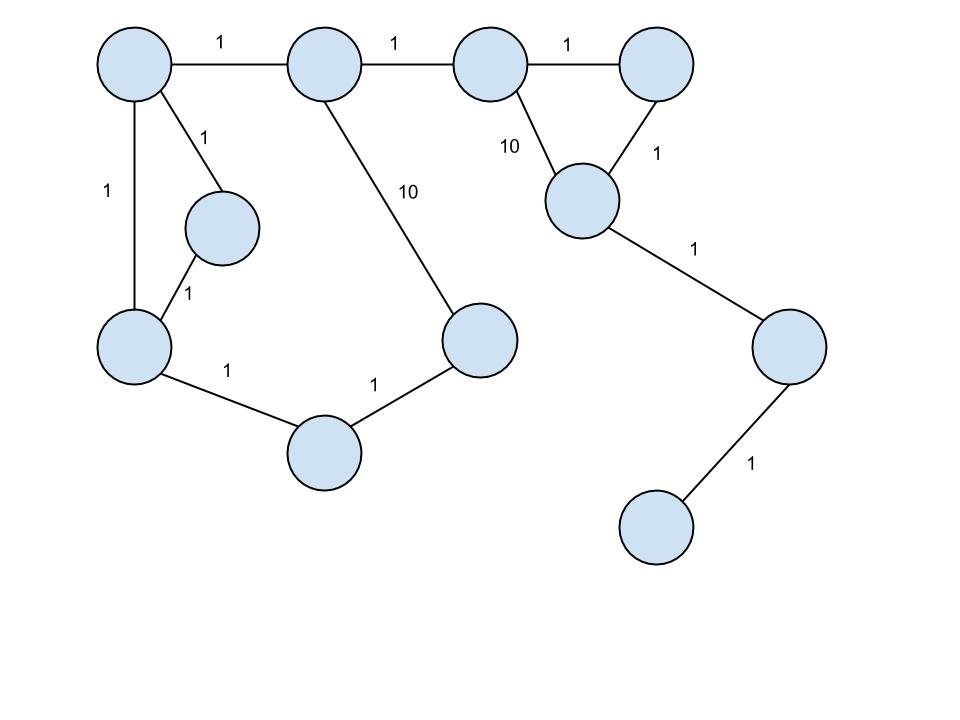
\includegraphics[scale=0.25]{imagenes/anillo-sin-hacer.jpg}
  \end{center}
  \caption{ejemplo de configuración de PCs y enlaces (con sus correspondientes costos).}
\end{figure}

La solución óptima consiste en crear un anillo utilizando únicamente los
enlaces de costo 1 y dejar el resto de la red conectada de la siguiente
forma:

\begin{figure}[htb]
  \begin{center}
      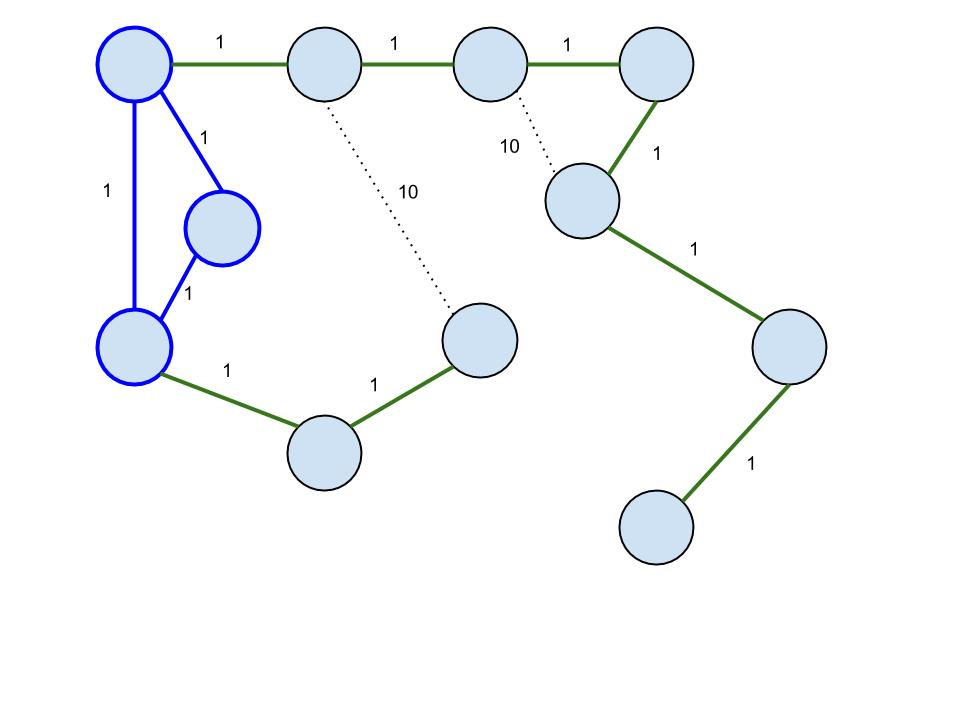
\includegraphics[scale=0.25]{imagenes/anillo-hecho.jpg}
  \end{center}
  \caption{ejemplo de anillo realizado.}
\end{figure}


\newpage
\subsection{Desarrollo de la idea y pseudocódigo.}

\vspace*{0.3cm}

En este problema, \textbf{trataremos a la red de computadoras como un grafo},
donde \textbf{las computadoras serán los vértices, las conexiones las aristas
y el peso de cada arista será el costo de hacer dicha conexión}.

Comenzaremos por corroborar que exista una solución. Para esto \textbf{el
grafo deberá ser conexo} y para cumplir con esto, debe tener \textbf{al
menos tantas aristas como vértices}. Si no fuese conexo, no se podrían
unir todas las computadoras. \textbf{Si tiene menos aristas que vértices},
el grafo sería un árbol y \textbf{nunca podría formarse un anillo}.

Suponiendo que tiene solución, se procederá a calcular el \textbf{árbol
generador mínimo} mediante el \textbf{algoritmo de Prim}. Para obtener el
anillo, \textbf{formaremos un ciclo agregando la arista de menor peso} no
incluída en el \textit{AGM}.


\begin{codebox}
\Procname{$\proc{sePuedeAnillar}(G)$}
\li \If $\neg (\proc{tieneSolucion}(G))$
\li     \Then
            \Return $\const{false}$
        \End
\li $\proc{completarAnillo}(\proc{Prim}(G,w,r),G)$
\li \Return $\const{true}$
\end{codebox}


\vspace*{0.3cm}


\begin{codebox}
\Procname{$\proc{tieneSolucion}(G)$}
\li \Return $(\proc{esConexo}(G,v)) \land
    \proc{\#}(\proc{aristas}(G)) \geq
    \proc{\#}(\proc{nodos}(G))$
\end{codebox}


\vspace*{0.3cm}


\begin{codebox}
\Procname{$\proc{Prim}(G,w,r)$}
\li \Comment $\id{u}$ es un nodo cualquiera de \id{G}.
\li \For $each \hspace{0.07cm} \id{u} \in \id{G.V}$
\li     \Do
            $\id{u.clave} \gets \infty$
\li         $\id{u.\pi} \gets \const{nil}$
        \End
\li $\id{r.clave} \gets 0$
\li $\id{Q} \gets \id{G.V}$
\li \While $\id{Q} \neq 0$
\li     \Do
            $\id{u} \gets \proc{extraerMinimo}(Q)$
\li         \For $each \hspace{0.07cm} \id{v} \in \id{G.Ady[u]}$
                \Do
\li                 \If $\id{v} \in \id{Q} \land (\id{w(u,v)} < \id{v.clave})$
\li                     \Then
                            $\id{v.\pi} \gets \id{u}$
\li                         $\id{v.clave} \gets \id{w(u,v)}$
                        \End
                \End
        \End
\end{codebox}


\vspace*{0.3cm}


\begin{codebox}
\Procname{$\proc{esConexo}(G,v)$}
\li \Comment $\id{u}$ es un nodo cualquiera de \id{G}.
\li \For $each \hspace{0.07cm} \id{u} \in \id{G.V}$
\li     \Do
            $\id{u.color} \gets \const{blanco}$
\li         $\id{u.d} \gets \infty$
\li         $\id{u.\pi} \gets \const{nil}$
        \End
\li $\id{s.color} \gets \const{gris}$
\li $\id{s.d} \gets 0$
\li $\id{s.\pi} \gets \const{nil}$
\li $\id{Q} \gets \emptyset$
\li \While $\id{Q} \neq 0$
\li     \Do
            $\id{u} \gets \proc{desencolar}(Q)$
\li         \For $each \hspace{0.07cm} \id{v} \in \id{G.Ady[u]}$
                \Do
\li                 \If $\id{v.color} \isequal \const{blanco}$
\li                     \Then
                            $\id{v.color} \gets \const{gris}$
\li                         $\id{v.d} \gets \id{u.d + 1}$
\li                         $\id{v.\pi} \gets \id{u}$
\li                         $\proc{encolar}(Q,v)$
                        \End
                \End
\li     $\id{u.color} \gets \const{negro}$
        \End
\end{codebox}


\vspace*{0.3cm}


\begin{codebox}
\Procname{$\proc{completarAnillo}(AGM, G)$}
\li $\id{X} \gets \proc{aristas}(G) \setminus \proc{aristas}(AGM)$
\li $\id{m} \gets \proc{dameUno}(X)$
\li $\id{X} \gets \id{X} \setminus \{m\}$
\li \While $\neg (\proc{vacio}(X))$
\li     \Do
\           $\id{y} \gets \proc{dameUno}(X)$
\li         \If $\proc{peso}(y) < \proc{peso}(m)$
\li             \Then
                    $\id{m} \gets \id{y}$
                \End
\li         $\id{X} \gets \id{X} \setminus \{y\}$
        \End
\li \Return $\proc{agregar}(AGM, m)$
\end{codebox}



\newpage
\subsection{Justificación de la resolución y demostración de correctitud.}

\vspace*{0.3cm}

\textcolor{red}{\textbf{completar!}}



\newpage
\subsection{Análisis de complejidad.}

\vspace*{0.3cm}

\textcolor{red}{\textbf{completar!}}



\newpage
\subsection{Experimentación y gráficos.}

\vspace*{0.3cm}

\subsubsection{Test 1 - benchmark caso aleatorio}

\textcolor{red}{\textbf{completar!}}


\newpage
\subsubsection{Test 2 - benchmark del peor caso}

\textcolor{red}{\textbf{completar!}}


\newpage
\subsubsection{Test 3 - benchmark del mejor caso}

\textcolor{red}{\textbf{completar!}}
